\section{Gathering Human Feedback}
\label{sec:gather-feedback}

In this section, we explore the process of gathering human feedback for aligning large language models (LLMs) with human values. To identify what "alignment" means, we first need to clarify what is meant by "alignment". According to the OpenAI InstructGPT paper \cite{ouyangTrainingLanguageModels2022}, the definition of alignment is the ability of the model to generate text responses which are: 
\begin{itemize}
    \item Helpful
    \item Honest
    \item Harmless
\end{itemize}

Here the definition of "helpful" agent is the ability of the model to generate outputs that follow instruction, but also provide helpful,as intended by user, (helpful to user). Measuring the "honesty" and the "harmlessness" of the model's output as well is difficult. In the work of \cite{ouyangTrainingLanguageModels2022}, the authors used two metrics to evaluate the honesty and harmlessness of the model's output. The first metric is to evaluate models tendency 
to make up information "hallucination" and the second metric is to evaluate the models using the benchmark
dataset like TruthfulQA dataset \cite{linTruthfulQAMeasuringHow2022}."Harmlessness" also
is a difficult metric to measure. The authors of \cite{ouyangTrainingLanguageModels2022} used
relied more on being "less toxic" as a metric to measure the harmlessness of the model's output.

To align LLMs output with these objectives (HHH), OpenAI employed 40 labelers via Upwork to provide feedback on model outputs. Demographic information about the labelers is presented in Figure \ref{fig:demograph}. 


\begin{figure}[h]
    \centering
    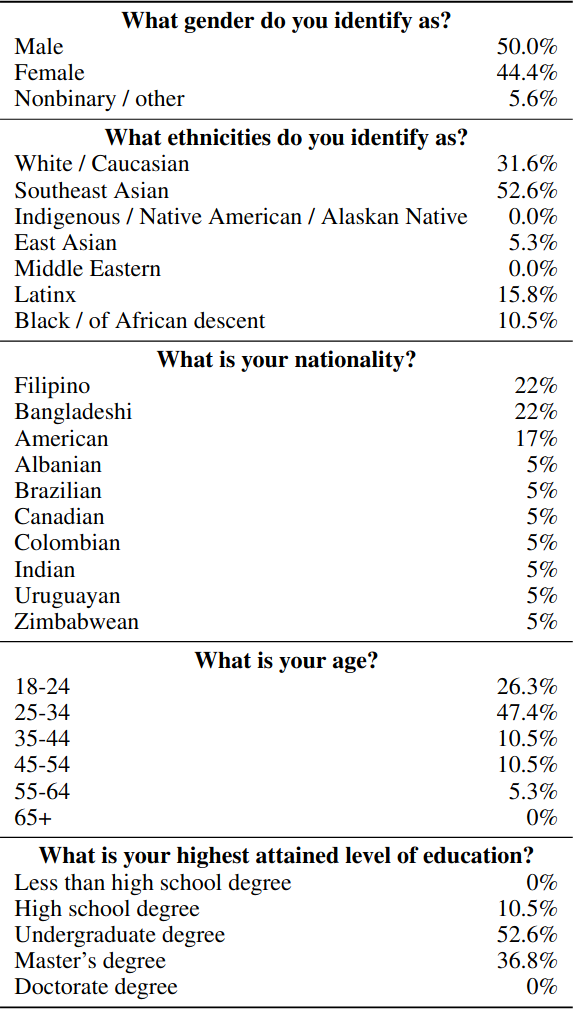
\includegraphics[width=0.6\textwidth]{./figures/demography1.png}
    \caption{Labelers demographic data in \cite{ouyangTrainingLanguageModels2022} work}
    \label{fig:demograph}
\end{figure}

\subsection{Feedback Gathering Interface} \label{subsec:feedback-interface}


Two example interfaces used to collect human feedback are presented here, illustrating how labelers (humans) give a feedback to the output of LLMs:\\




\begin{figure}[h]
    \centering
    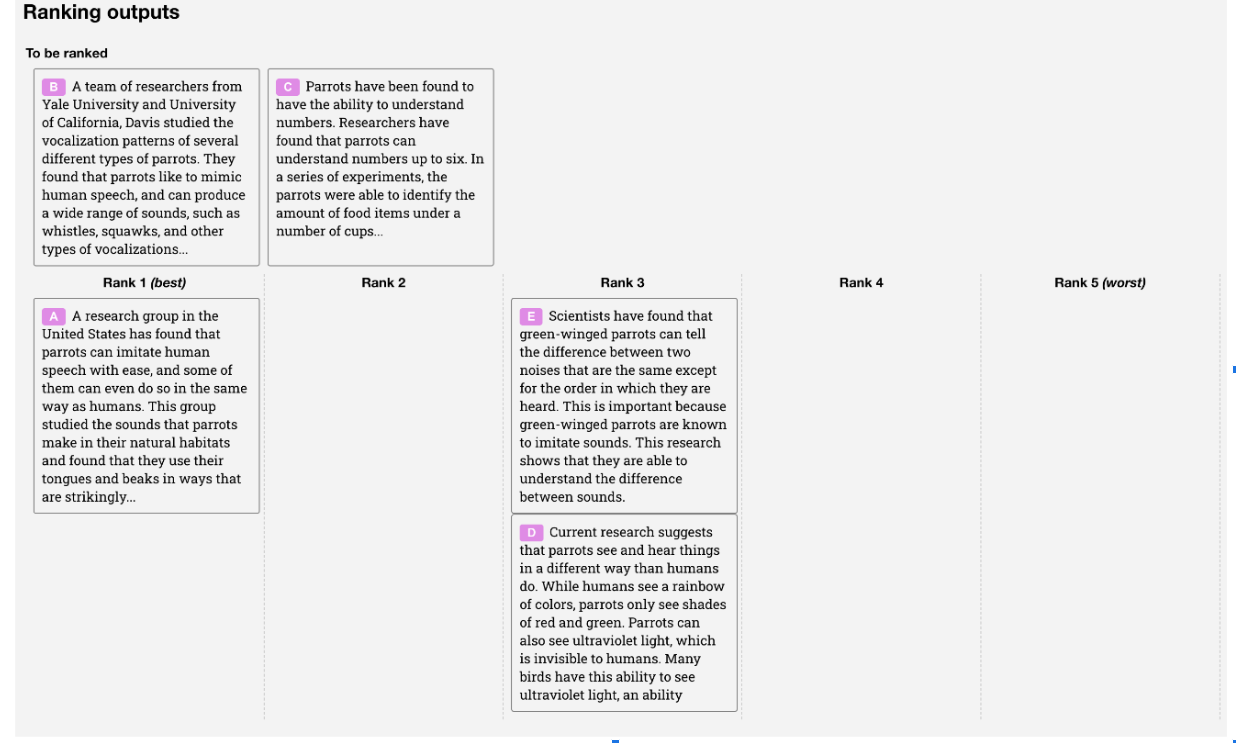
\includegraphics[width=0.8\textwidth]{./figures/image_interface_openai.png}
    \caption{OpenAI Feedback Interface}
    \label{fig:interface-openai}
\end{figure}

\textbf{OpenAI Feedback Interface}

The first interface is the interface used to gather feedback for InstructGPT model. As we can see from the Figure 
\ref{fig:interface-openai}, the LLM model generates 5 responses, and the labeler 
needs to select the best response and the worst response for the given prompt. In the Figure \ref{fig:interface-openai}, the prompt for the replies was "summarize the article". \\


\textbf{Anthropic Feedback Interface}


A similar process is employed by Anthropic for training their large language models in RLHF stage, as shown in Figure \ref{fig:interface-anthropic}. In this example, the feedback interface includes the dialogue history as context (state), with the pre-trained model generating two potential completions. Labelers are then tasked with selecting which text completion is better. This feedback is used to train the model further to align with human intent \cite{baiConstitutionalAIHarmlessness2022}. \\


\begin{figure}[h]
    \centering
    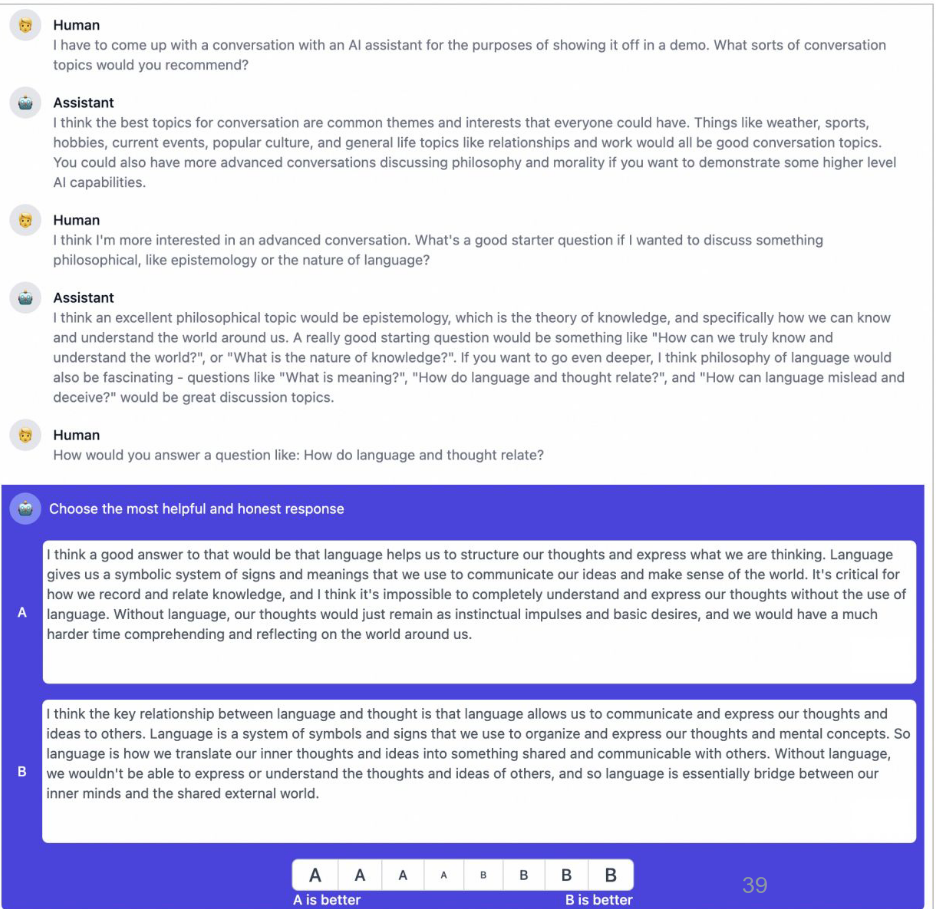
\includegraphics[width=0.8\textwidth]{./figures/interfcae_antropic.png}
    \caption{Anthropic Feedback Interface}
    \label{fig:interface-anthropic}
\end{figure}



In this section, we would like to highlight the concern raised by \cite{atariWhichHumans2023}, which discusses 
the importance of incorporating culturally diverse feedback to ensure LLMs are representative of global values, rather than being skewed towards Western, Educated, Industrialized, Rich, and Democratic (WEIRD) perspectives. Their analysis of current LLM performance revealed that these models align most closely with the preferences and behaviors of individuals from WEIRD societies, while their performance are significantly less correlated for populations outside this demographic.
